\documentclass[12pt,letterpaper,noanswers]{exam}
\usepackage[usenames,dvipsnames,svgnames,table]{xcolor}
\usepackage[margin=0.9in]{geometry}
\renewcommand{\familydefault}{\sfdefault}
\usepackage{multicol}
\pagestyle{head}
\header{AM 111 Class 06}{}{Linear least squares: $SVD$, p.\thepage}
\runningheadrule
\headrule
\usepackage{siunitx}
\usepackage{enumitem}
\usepackage{graphicx} % more modern
\usepackage{amsmath} 
\usepackage{amssymb} 
\usepackage{hyperref}

\usepackage[most]{tcolorbox}
\usepackage{listings}

\definecolor{white}{rgb}{1,1,1}
\definecolor{mygreen}{rgb}{0,0.4,0}
\definecolor{light_gray}{rgb}{0.97,0.97,0.97}
\definecolor{mykey}{rgb}{0.117,0.403,0.713}

\tcbuselibrary{listings}
\newlength\inwd
\setlength\inwd{1.3cm}
% https://tex.stackexchange.com/questions/340700/ipython-notebook-input-and-output-cells-with-listings
\newcounter{ipythcntr}
\renewcommand{\theipythcntr}{\texttt{[\arabic{ipythcntr}]}}

\newtcblisting{pyin}[1][]{%
  sharp corners,
  enlarge left by=\inwd,
  width=\linewidth-\inwd,
  enhanced,
  boxrule=0pt,
  colback=light_gray,
  listing only,
  top=0pt,
  bottom=0pt,
  overlay={
    \node[
      anchor=north east,
      text width=\inwd,
      font=\footnotesize\ttfamily\color{mykey},
      inner ysep=2mm,
      inner xsep=0pt,
      outer sep=0pt
      ] 
      at (frame.north west)
      {\refstepcounter{ipythcntr}\label{#1}In \theipythcntr:};
  }
  listing engine=listing,
  listing options={
    aboveskip=1pt,
    belowskip=1pt,
    basicstyle=\footnotesize\ttfamily,
    language=Python,
    keywordstyle=\color{mykey},
    showstringspaces=false,
    stringstyle=\color{mygreen}
  },
}
\newtcblisting{pyprint}{
  sharp corners,
  enlarge left by=\inwd,
  width=\linewidth-\inwd,
  enhanced,
  boxrule=0pt,
  colback=white,
  listing only,
  top=0pt,
  bottom=0pt,
  overlay={
    \node[
      anchor=north east,
      text width=\inwd,
      font=\footnotesize\ttfamily\color{mykey},
      inner ysep=2mm,
      inner xsep=0pt,
      outer sep=0pt
      ] 
      at (frame.north west)
      {};
  }
  listing engine=listing,
  listing options={
      aboveskip=1pt,
      belowskip=1pt,
      basicstyle=\footnotesize\ttfamily,
      language=Python,
      keywordstyle=\color{mykey},
      showstringspaces=false,
      stringstyle=\color{mygreen}
    },
}
\newtcblisting{pyout}[1][\theipythcntr]{
  sharp corners,
  enlarge left by=\inwd,
  width=\linewidth-\inwd,
  enhanced,
  boxrule=0pt,
  colback=white,
  listing only,
  top=0pt,
  bottom=0pt,
  overlay={
    \node[
      anchor=north east,
      text width=\inwd,
      font=\footnotesize\ttfamily\color{mykey},
      inner ysep=2mm,
      inner xsep=0pt,
      outer sep=0pt
      ] 
      at (frame.north west)
      {\setcounter{ipythcntr}{\value{ipythcntr}}Out#1:};
  }
  listing engine=listing,
  listing options={
      aboveskip=1pt,
      belowskip=1pt,
      basicstyle=\footnotesize\ttfamily,
      language=Python,
      keywordstyle=\color{mykey},
      showstringspaces=false,
      stringstyle=\color{mygreen}
    },
}





\newcommand{\note}[1]{\textcolor{red}{#1}} % show notes in red
\renewcommand{\note}[1]{} % don't display notes

\begin{document}
 \pdfpageheight 11in 
  \pdfpagewidth 8.5in


  
\section{Preliminaries}
\begin{itemize}
\itemsep0pt
\item Problem set 02 is due on Friday at noon.
\item Problem set 02 includes some ``time permitting'' problems.  If your time spent on the problem set reaches 8 hours in the week then you are encouraged to skip these problems.  If you are not in that situation, you are expected to complete the problems.
\item There will be a skill check in class during Class 07.  The problem info is below.
\end{itemize}



\noindent\textbf{Big picture}

Using linear least squares data fitting leads to a matrix equation.  Once that is set up, we can construct the normal equations or can use matrix decomposition to solve.

Today: solving via $SVD$ decomposition.

\vspace{0.2cm}
\hrule
\vspace{0.2cm}
\noindent \textbf{Skill check practice}
\begin{questions}
\item Given a matrix $A$ (where $A^TA$ is diagonal), find the singular values of $A$.

Example: Find the singular values of $A = \left[\begin{array}{r r}
-4 & 1 \\
1 & 4 \\
0 & 2
\end{array}\right]$

\end{questions}


\vspace{0.2cm}
\hrule
\vspace{0.2cm}

\noindent \textbf{Skill check solution}
\begin{questions}
\item $A = \left[\begin{array}{r r}
-4 & 1 \\
1 & 4 \\
0 & 2
\end{array}\right]$ so $A^TA = \left[\begin{array}{r r r}
-4 & 1 & 0 \\
1 & 4 & 2
\end{array}\right]\left[\begin{array}{r r}
-4 & 1 \\
1 & 4 \\
0 & 2
\end{array}\right] = \left[\begin{array}{r r}
17 & 0 \\
0 & 21
\end{array}\right]$.

The eigenvalues of a diagonal matrix are given by the diagonal entries: $17, 21$.  The singular values of $A$ are the square roots of the eigenvalues of $A^TA$ so are $\sqrt{17}, \sqrt{21}$.

\end{questions}

\section{Solving the least squares problem}

\subsection{Matrix decomposition: $SVD$}

We will use one more matrix decomposition to solve the least squares problem.

\subsubsection{The singular values}
See Lay \S 7.4, Heath \S 3.6, \S 4.7, Sauer \S 12.3

Recall that a matrix is a mapping between two vector spaces.

Example: $A$ be $10\times 2$.  $A$ maps vectors in $\mathbb{R}^{10}$ to vectors in $\mathbb{R}^2$.

Consider the length of $A\mathbf{v}$, the mapping of $\mathbf{v}$ into $\mathbb{R}^{10}$.

$\Vert A\mathbf{v}\Vert^2 = \mathbf{v}^TA^TA\mathbf{v}$ where $A^TA$ is a symmetric matrix.

Symmetric matrices have a number of nice properties.  They can be orthogonally diagonalized.  Let $\mathbf{v}_i$ be an eigenvector of $A^TA$ with unit length.

$\Vert A\mathbf{v}_i\Vert^2 = \mathbf{v}_i^T\lambda_i\mathbf{v}_i = \lambda_i$ ($\mathbf{v}_i$ has unit length).

So $\Vert A\mathbf{v}_i\Vert = \sqrt{\lambda_i}$.  

Def: The singular values, $\sigma_i$, are the square roots of the eigenvalues of $A^TA$ arranged in descending order.  

Note: the singular values are the lengths of the vectors $A\mathbf{v}_1,..,A\mathbf{v}_n$.

Theorem: Suppose $\mathbf{v}_1,...,\mathbf{v}_n$ is an orthnonormal basis of $\mathbb{R}^n$ consisting of eigenvectors of $A^TA$ arranged so that the corresponding eigenvalues are in descending order.  Suppose $A$ has $r$ nonzero singular values.  Then $\left\{A\mathbf{v}_1,...,A\mathbf{v}_r\right\}$ is an orthogonal basis for the columns space of $A$, and rank $A= r$.

Proof: $(A\mathbf{v}_i)^T(A\mathbf{v}_j) = \mathbf{v}_i^T\lambda_i\mathbf{v}_j = 0$ (for $i\neq j$).  So they are an orthogonal set.  And there are $r$ vectors in the set.  If $\mathbf{y} = A\mathbf{x}$ then $\mathbf{x} = c_1\mathbf{v}_1 + ... +c_n\mathbf{v}_n$ but $A\mathbf{x} = c_1A\mathbf{v}_1 + ... + c_r A\mathbf{v}_r$ so $\mathbf{y}$ is in the span of the $r$ vectors.

\begin{enumerate}
\item Which of the following matrices are orthogonal? (Heath 3.23)
\begin{parts}
\item $\left[\begin{array}{r r}
0 & 1 \\ 1 & 0
\end{array}\right]$
\item $\left[\begin{array}{r r}
1 & 0 \\ 0 & -1
\end{array}\right]$
\item $\left[\begin{array}{r r}
2 & 0 \\ 0 & 1/2
\end{array}\right]$
\item $\left[\begin{array}{r r}
\sqrt{2}/2 & \sqrt{2}/2 \\ -\sqrt{2}/2 & \sqrt{2}/2
\end{array}\right]$
\end{parts}

\item Show that the columns of $U$ are eigenvectors of $AA^T$.
\end{enumerate}


\subsubsection{Reduced singular value decomposition}

Let $A\mathbf{c} = \mathbf{y}$ be overdetermined with $A$ full rank.  $A$ is $m\times n, m>n$ so rank$(A) = n$.

$A = U_1 S_1 V^T$ where $V = \left[\mathbf{v}_1 ... \mathbf{v}_n\right]$, $S = \left[\begin{array}{l r r r l}\sigma_1 & 0 & ... & & 0\\
0 & \sigma_2 & 0 & ... & 0 \\
\vdots & & \ddots & & \vdots \\
\\
0 & ... & & 0 & \sigma_n\end{array}\right]$, and $U_1 = \left[\mathbf{u}_1 ... \mathbf{u}_n \right]$

where $\mathbf{u}_i = \dfrac{1}{\sigma_i}A\mathbf{v}_i$

The $\mathbf{u}_i$ are called left singular vectors and the $\mathbf{v}_i$ are called right singular vectors.

The matrix $A^+ = VS_1^{-1}U_1^T$ is called the pseudoinverse of $A$.



Given the reduced SVD for $A$ and the least squares problem
$A\mathbf{c} = \mathbf{y}$, we have
$\overline{\mathbf{c}} = VS_1^{-1}U_1^T\mathbf{y}$ $=\sum\limits_{\sigma_i\neq 0} \dfrac{1}{\sigma_i}(\mathbf{u}_i^T\mathbf{y})\mathbf{v}_i$




Note: Algorithms for computing the SVD avoid forming $A^TA$ or $AA^T$ and work directly with $A$ (to reduce numerical error).


\begin{enumerate}[resume]


\item Consider the column vector $\mathbf{a}$ as an $n\times 1$ matrix.  Write out its reduced singular value decomposition, finding $U_1, S_1, V$ explicitly.

\item Consider the row vector $\mathbf{a}^T$.  Why won't $\mathbf{a}^T$ have a reduced singular value decomposition?

\item Consider the figure below.  Which image represents the error in linear least squares?  What are the other two images showing?


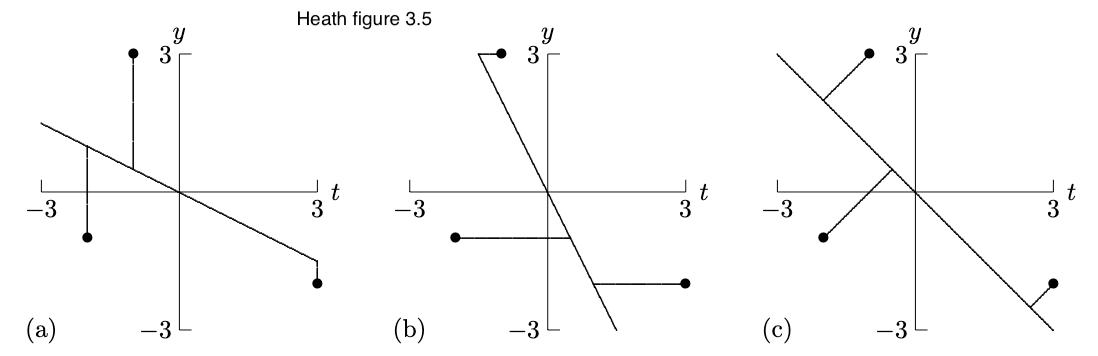
\includegraphics[width=\textwidth]{AM111-F23-CourseNotes/img/leastsquares.png}
\end{enumerate}


\begin{pyin}
\## 21 microseconds
U1, S1, VT = np.linalg.svd(A, full_matrices=False)
sigma = np.diag(S1)
# pseudoinverse of sigma:
sigma_inv = np.linalg.pinv(sigma)
c_over = VT.T @ sigma_inv @ U1.T @ y
print("coefficients:", [c for c in c_over])
\end{pyin}
\begin{pyout}
coefficients: [1.         1.         1.         0.99999999 1.00000004 1.00000003 1.00000006 1.        ]
\end{pyout}

\begin{pyin}
\## 13.9 microseconds
c_over, res, rnk, s = linalg.lstsq(A, y)
print("coefficients:", [c for c in c_over])
\end{pyin}
\begin{pyout}
coefficients: [1.         1.         1.         1.         1.         1.00000001 0.99999999 1.00000001]
\end{pyout}



% \subsection{Other SVD facts}


% In the Euclidean norm, the matrix condition number is given by $\text{cond}(A) = \sigma_{max}/\sigma_{min}$.


\section{Total least squares}

For $A\mathbf{c}= \mathbf{y}$ we have been assuming that the entries of $A$ are exactly correct, while the entries in $\mathbf{y}$ are a little off from our model.

We minimize $\Vert \mathbf{y} - \mathbf{a}\Vert$ where $\mathbf{a}\in\text{span}(A)$.  

For total least squares, allow the matrix to vary as well.

Consider the matrix $[A\ \mathbf{y}]$.  It is an $m \times (n+1)$ matrix.  Let $[\hat{A}\ \mathbf{a}]$ be an approximating system that is compatible, so $\mathbf{a}\in\text{span}(\hat{A})$.  This approximating system needs to have rank $n$.

A solution of a compatible system must satisfy $[\hat{A} \ \mathbf{a}]\left[\begin{array}{r} \mathbf{c} \\ -1 \end{array}\right] = \mathbf{0}$.

That means $\left[\begin{array}{r} \mathbf{c} \\ -1 \end{array}\right]$ is in the null space of $[\hat{A} \ \mathbf{a}]$.

Set $\left[\begin{array}{r} \mathbf{c} \\ -1 \end{array}\right]$ proportional to $\mathbf{v}_{n+1}$ with $[\hat{A} \ \mathbf{a}]$ created by using the first $n$ singular values.  This approximation satisfies the conditions.


\begin{enumerate}[resume]
\item Find the line of code where the coefficients are constructed.  What are the steps to create the vector $\mathbf{c}$?

\begin{pyin}
\## 9.4 microseconds
A1 = np.column_stack((A, y))
U1, S1, VT = np.linalg.svd(A1, full_matrices=False)
c_over_2 = -1/VT.T[-1,-1]*VT.T[0:-2,-1]
print("coefficients:", [c for c in c_over_2])

S1[-1] = 0
sigma = np.diag(S1)
Ahat = U1@sigma@VT
\end{pyin}

\begin{pyout}
coefficients: [1. 1.  1.  1. 1. 1. 0.99999999]
\end{pyout}

\end{enumerate}

\section{More practice}


\begin{enumerate}[resume]
\item T/F: In solving a linear least squares problem $A\mathbf{c} = \mathbf{y}$ if the vector $\mathbf{y}$ lies in $\text{span}(A)$ then the error vector is $\mathbf{0}$.
\item Give an example of a model function that is non-linear in the components of $\mathbf{c}$.
\item For an overdetermined least squares problem, which is more serious: the rows of $A$ are linearly dependent, or the columns of $A$ are linearly dependent?
\item Let $\overline{\mathbf{c}}$ be the least squares  solution to $A\mathbf{c} = \mathbf{y}$ where $A = \left[\begin{array}{c c} 1 & 0 \\
1 & 1 \\
1 & 2 \\
 1 & 3\end{array}\right]$

Let $\mathbf{r} = \mathbf{y} - A\overline{\mathbf{c}}$.

Consider the vector $\left[\begin{array}{r}-1 \\ -1 \\ 1 \\ 1\end{array}\right].$  Why isn't this a possible value of $\mathbf{r}$?

Construct a vector that is a possible value of $\mathbf{r}$.
 
\end{enumerate}
\end{document}